\documentclass[b5paper,openany]{standalone}
\usepackage{luatexja-preset}
\usepackage{xcolor}
\usepackage{tikz}
\usetikzlibrary{calc}
\usetikzlibrary{positioning}
\usetikzlibrary{arrows.meta}
\usetikzlibrary{shapes.geometric}
\begin{document}
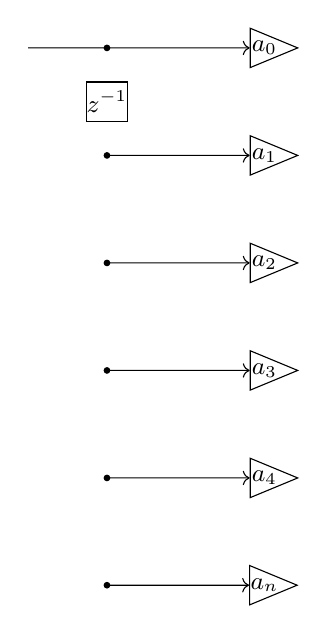
\begin{tikzpicture}[scale=1]
  \tikzset{every node/.style={shape=circle,font=\small,text centered,inner sep=0pt,minimum size=0.5cm}};
  \node [isosceles triangle, draw] (a0) {$a_0$};
  \node [isosceles triangle, draw, below=of a0] (a1) {$a_1$};
  \node [isosceles triangle, draw, below=of a1] (a2) {$a_2$};
  \node [isosceles triangle, draw, below=of a2] (a3) {$a_3$};
  \node [isosceles triangle, draw, below=of a3] (a4) {$a_4$};
  \node [isosceles triangle, draw, below=of a4] (an) {$a_n$};
  \path[draw] ($(a0)+(-3cm,0)$) -- +(1cm,0) coordinate (con0) [fill]circle(1pt) [arrows=->]edge (a0.west);
  \path[draw] ($(a1)+(-2cm,0)$) coordinate (con1) [fill]circle(1pt) [arrows=->]edge (a1.west);
  \path[draw] ($(a2)+(-2cm,0)$) coordinate (con2) [fill]circle(1pt) [arrows=->]edge (a2.west);
  \path[draw] ($(a3)+(-2cm,0)$) coordinate (con3) [fill]circle(1pt) [arrows=->]edge (a3.west);
  \path[draw] ($(a4)+(-2cm,0)$) coordinate (con4) [fill]circle(1pt) [arrows=->]edge (a4.west);
  \path[draw] ($(an)+(-2cm,0)$) coordinate (conn) [fill]circle(1pt) [arrows=->]edge (an.west);
  \path[draw]  ($(con0)!0.5!(con1)$) node[draw,rectangle] {$z^{-1}$};
\end{tikzpicture}
\end{document}
